\documentclass{report}

\newcommand{\Alpha}{A}

\usepackage[french]{babel}
\usepackage[T1]{fontenc}
\usepackage[utf8]{inputenc}
\usepackage{fontspec}
\usepackage[left=0.60in, right=0.60in, top=1.5in, bottom=0.50in, nohead, includefoot]{geometry}
\usepackage{scrextend}
\usepackage{listings}
\usepackage[hidelinks,unicode=true]{hyperref}
\usepackage[pgf]{dot2texi}
\usepackage{pgf}
\usepackage{tikz}
\usepackage{sectsty}
\usepackage{titlesec}
\usepackage{csquotes}
\usepackage{hyperref}
\usepackage{keystroke}
\usepackage{booktabs}
\usepackage{color, colortbl}
\usepackage[labelformat=empty]{caption}
\usepackage{framed}
\usepackage{amsmath}
\usepackage[linguistics]{forest}
\usepackage{adjustbox}
\usepackage{afterpage}

\setcounter{tocdepth}{4}
\setcounter{secnumdepth}{4}

\renewcommand*{\thefootnote}{(\arabic{footnote})}

\hypersetup{
  colorlinks = true,
  linkcolor = blue,
  urlcolor = blue,
}

\usetikzlibrary{automata, shapes, arrows, snakes, matrix, positioning}

\setmainfont[
	Path = assets/fonts/,
	Extension = .ttf,
	Ligatures = TeX,
	Scale = MatchLowercase,
]{sazanami-mincho}

\setsansfont[
	Path = assets/fonts/,
	Extension = .ttf,
	Ligatures = TeX,
	Scale = MatchLowercase,
]{sazanami-gothic}

\pagenumbering{gobble}

\title{}

\author{
   adjivas
   \and
   jb
}

\date{}

\begin{document}

\afterpage{
    \begin{figure}[!ht]
        \begin{center}
            \Huge \textbf{
                \fontsize{60pt}{60pt}\fontspec[Path = assets/fonts/, Extension = .ttf, Ligatures = TeX]{tetris}{Dot-Machine}
            } \\
            \vspace{0.75ex}
            \footnotesize \href{https://jb255.github.io/Dot-machine/}{jb255.github.io/Dot-machine} \\
            \vspace{24ex}
            \begin{tikzpicture}
                \node[anchor=south west,inner sep=0] (image) at (0,0,0) {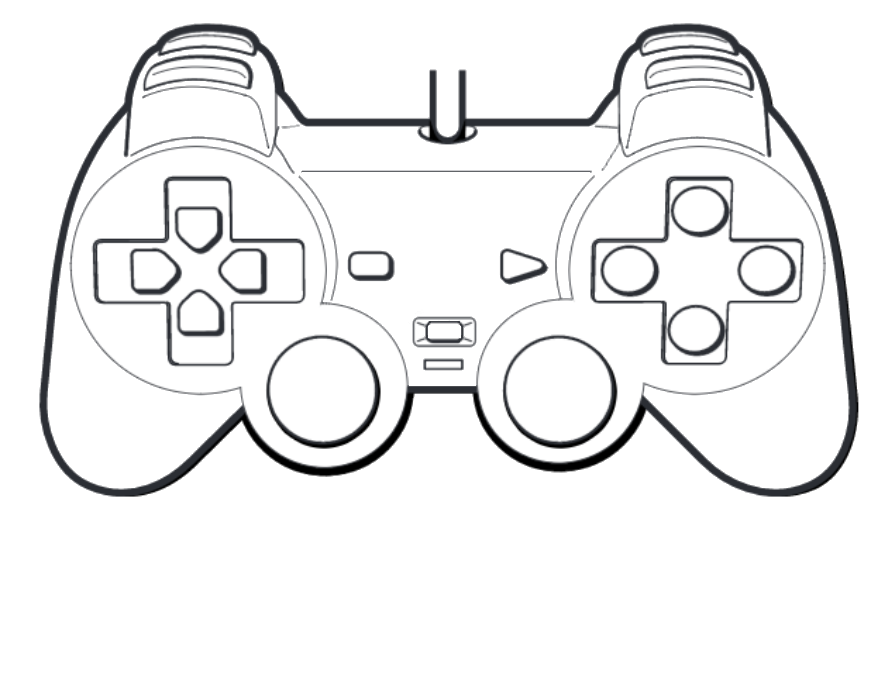
\includegraphics[scale=0.25]{assets/images/pad.png}};
                \begin{scope}[x={(image.south east)},y={(image.north west)}]

                    % Select
                    \draw[color=gray, *-] (0.58, 0.6) -- (0.58, 1) node[anchor=south] {tetris};
                    % Start
                    %\draw[color=gray, *-] (0.42, 0.6) -- (0.42, 1) node[anchor=south] {tetris};

                    % L
                    \draw[color=gray, *-] (0.25, 0.93) -- (0.25, 1) node[anchor=south] {son};
                    \draw[color=gray, *-] (0.2, 0.90) -- (0, 0.90) -- (0, 1) node[anchor=south] {chute};

                    % R
                    %\draw[color=gray, *-] (0.75, 0.93) -- (0.75, 1) node[anchor=south] {};
                    %\draw[color=gray, *-] (0.8, 0.90) -- (1, 0.90) -- (1, 1) node[anchor=south] {};

                    % top
                    \draw[color=gray, *-] (0.234, 0.674) -- (0, 0.674) -- (0, 0.79) -- (-0.1, 0.79) node[anchor=east] {rotation};
                    % right
                    \draw[color=gray, *-] (0.18, 0.605) -- (-0.1, 0.605) node[anchor=east] {gauche};
                    % bottom
                    \draw[color=gray, *-] (0.229, 0.55) -- (0.229, 0.445) -- (-0.1, 0.445) node[anchor=east] {bas};
                    % left
                    \draw[color=gray, *-] (0.28, 0.62) -- (0.28, 0.27) -- (-0.1, 0.27) node[anchor=east] {droite};

                    % triangle
                    \draw[color=gray, *-] (0.775, 0.69) -- (1, 0.69) -- (1, 0.79) -- (1.1, 0.79) node[anchor=west] {rotation adverse};
                    % circle
                    \draw[color=gray, *-] (0.852, 0.605) -- (1.1, 0.605) node[anchor=west] {droite adverse};
                    % cross
                    \draw[color=gray, *-] (0.78, 0.53) -- (0.78, 0.445) -- (1.1, 0.445) node[anchor=west] {bas adverse};
                    % square
                    \draw[color=gray, *-] (0.705, 0.62) -- (0.705, 0.275) -- (1.1, 0.275) node[anchor=west] {gauche adverse};
                \end{scope}
            \end{tikzpicture}
            \caption[Caption for LOF] {
	            \begin{tabular}{p{.30\textwidth}p{.65\textwidth}}
	                \toprule
	                \toprule
		            $PS_X$ & $Description$ \\
	                \midrule
                    \keystroke{Start} & Lancer ou relancer une partie. \\
                    \keystroke{L2} & Active ou désactive le son. \\
                    \keystroke{L1} & Chuter la pièce. \\
                    \UArrow{} & Tourner la pièce. \\
                    \RArrow{} & Déplacer la pièce vers la droite. \\
                    \LArrow{} & Déplacer la pièce vers la gauche. \\
                    \DArrow{} & Déplacer la pièce vers le bas. \\
                    \keystroke{
\includegraphics[scale=0.5]{assets/images/PlayStationTriangle.png}} & Tourner la pièce adverse\footnotemark[1]. \\
                    \keystroke{
\includegraphics[scale=0.5]{assets/images/PlayStationCircle.png}} & Déplacer la pièce adverse vers la droite\footnotemark[1]. \\
                    \keystroke{
\includegraphics[scale=0.5]{assets/images/PlayStationSquare.png}} & Déplacer la pièce adverse vers la gauche\footnotemark[1]. \\
                    \keystroke{
\includegraphics[scale=0.5]{assets/images/PlayStationX.png}} & Déplacer la pièce adverse vers le bas\footnotemark[1]. \\
	                \bottomrule
	            \end{tabular}
            }
        \end{center}
    \end{figure}
    \footnotetext[1]{Les déplacements de la pièce adverses nécessitent des points bonus qui seront gagnés par la complétion de lignes.}
}
    
\end{document}
